% ============================================================================
% HACE: Addressing Viability Failure in Sequential Reinforcement Learning
%       with Homeostatic Auxiliary Rewards
%
% CSCI 2951X Course Project — Spring 2026
% Brown University
%
% To compile:
%   pdflatex main.tex && bibtex main && pdflatex main.tex && pdflatex main.tex
% ============================================================================

\documentclass[sigplan,10pt]{acmart}

\settopmatter{printfolios=false,printacmref=false}
\setcopyright{none}
\acmConference[CSCI 2951X]{CSCI 2951X Course Project}{Spring 2026}{Providence, RI, USA}
\acmYear{2026}
\acmDOI{}
\acmISBN{}
\acmPrice{}

% ── Packages ─────────────────────────────────────────────────
\usepackage{booktabs}
\usepackage{enumitem}
\usepackage{amsmath,amssymb}
\usepackage{algorithm}
\usepackage{algorithmic}
\usepackage{multirow}
\usepackage{subcaption}
\usepackage{xcolor}
\usepackage{hyperref}

% ── Notation shortcuts ───────────────────────────────────────
\newcommand{\setpoint}{H^*}
\newcommand{\energy}{E}
\newcommand{\drive}{d}
\newcommand{\reward}{r}
\newcommand{\hace}{\textsc{Hace}}

% ============================================================================
\begin{document}

\title{HACE: Addressing Viability Failure in Sequential Reinforcement Learning\\
with Homeostatic Auxiliary Rewards}

\newcommand{\browncsaffiliation}{%
  \affiliation{%
    \department{Department of Computer Science}
    \institution{Brown University}
    \city{Providence}
    \state{RI}
    \country{USA}}}

\author{Ziyu Kong}
\browncsaffiliation
\email{ziyu\_kong@brown.edu}

\author{Shihang Gui}
\browncsaffiliation
\email{shihang\_gui@brown.edu}

\author{Ruth Ukubay}
\browncsaffiliation
\email{ruth\_ukubay@brown.edu}

\author{Meiyi Song}
\browncsaffiliation
\email{meiyi\_song1@brown.edu}

% ============================================================================
\begin{abstract}
% ============================================================================

Continual reinforcement learning (CRL) research has focused almost
exclusively on \emph{catastrophic forgetting}---the tendency for neural
networks to lose previously acquired skills when adapting to new tasks.
In embodied settings where agents manage shared physiological resources
such as energy, we identify a complementary and equally critical failure
mode: \emph{viability failure}, wherein agents deplete internal resources
and die before they can learn a new task. We argue that established CRL
techniques such as Elastic Weight Consolidation (EWC), Experience Replay
(ER), and L2 regularization are structurally incapable of addressing
viability failure because it is a \emph{reward-level survival} problem,
not a parameter-preservation problem. We propose \hace{}
(Homeostatic Auxiliary for Continual Environments), a simple,
task-invariant auxiliary reward based on homeostatic drive reduction that
incentivizes energy management without requiring task-specific
engineering. We evaluate \hace{} alongside 8 baseline agents---including
EWC, ER, and L2 regularization---on a purpose-built 10-task sequential
gridworld benchmark with 3 curated task orderings and 2 boundary modes.
Our results demonstrate that (1)~\hace{} agents maintain viability
across task transitions, achieving 3--5$\times$ higher boundary
solvability than task-only baselines; (2)~traditional CRL methods fail
to prevent agent death at task boundaries and perform no better than
unprotected baselines on viability metrics; and (3)~\hace{} is
orthogonal to forgetting-prevention methods, with \hace{}+EWC addressing
both failure modes simultaneously. Our findings establish viability
maintenance as an essential and overlooked prerequisite for continual
embodied learning.

\end{abstract}

\maketitle

% ============================================================================
\section{Introduction}
\label{sec:intro}
% ============================================================================

Reinforcement learning agents deployed in sequential or continual settings
must adapt to changing objectives without losing previously learned
capabilities.  The dominant research paradigm in continual RL (CRL) frames
this challenge almost exclusively as \emph{catastrophic forgetting}---the
well-documented tendency for neural network parameters to overwrite old
knowledge when trained on new tasks~\cite{Parisi2019,kirkpatrick2017,continualworld2021}.
A rich toolkit of methods has emerged to combat forgetting: weight
regularization (EWC~\cite{kirkpatrick2017}), experience replay~\cite{rolnick2019},
progressive architectures~\cite{rusu2016}, and policy
distillation~\cite{rusu2015}.  These methods are evaluated almost exclusively
on whether old-task performance degrades after new-task training.

We argue that this singular focus on forgetting obscures an equally critical
failure mode that emerges naturally in \emph{embodied} sequential settings:
\textbf{viability failure}.  When an agent operates in an environment with
shared physiological constraints---such as an internal energy variable that
depletes with each action---the transition between tasks can be lethal.  An
agent that completes Task~$T_i$ with minimal remaining energy may arrive at
Task~$T_{i+1}$ without sufficient resources to survive long enough to learn.
No amount of EWC regularization or replayed transitions can save an agent that
dies in the first three steps of a new task.

Consider a concrete example from our benchmark.  An agent trained on
\textsc{Conservation} (high step cost, must be efficient) transitions to
\textsc{Sprint} (very short time limit, must be fast).  Under carryover
boundary conditions---where energy is not reset between tasks---a task-only
agent that learned conservative movement arrives at \textsc{Sprint} with
critically low energy and zero time to explore.  It dies immediately.  EWC
preserves the \textsc{Conservation} weights perfectly, but those weights are
useless if the agent cannot survive.

This paper makes three contributions:

\begin{enumerate}[leftmargin=*,topsep=2pt,itemsep=1pt]
  \item We formally identify \textbf{viability failure} as a distinct
        failure mode in continual embodied RL, separate from catastrophic
        forgetting, and show that traditional CRL methods are structurally
        unable to address it (Section~\ref{sec:viability}).

  \item We propose \textbf{\hace{}} (Homeostatic Auxiliary for Continual
        Environments), a simple, task-invariant auxiliary reward based on
        biological homeostatic drive reduction that incentivizes energy
        management across all tasks without task-specific engineering
        (Section~\ref{sec:hace}).

  \item We design a \textbf{10-task sequential gridworld benchmark} with
        12 structurally diverse tasks, 3 curated task orderings, 9 agent
        variants (including EWC, ER, L2, and oracle baselines), and 2
        boundary modes (reset/carryover) that enables systematic study
        of both forgetting and viability failure
        (Section~\ref{sec:benchmark}).
\end{enumerate}

Our experiments (Section~\ref{sec:experiments}) demonstrate that \hace{}
agents maintain viability across task boundaries, achieve higher boundary
solvability, and exhibit stronger forward transfer than both task-only
agents and standard CRL baselines.  Critically, \hace{} is
\emph{orthogonal} to forgetting-prevention methods: combining \hace{}
with EWC addresses both failure modes simultaneously.


% ============================================================================
\section{Related Work}
\label{sec:related}
% ============================================================================

\subsection{Continual Reinforcement Learning}

The CRL literature focuses on preventing catastrophic forgetting when an
agent's task changes over time.  Elastic Weight Consolidation
(EWC;~\cite{kirkpatrick2017}) slows updates to parameters deemed important
for previous tasks via a Fisher-weighted penalty.  Experience Replay
(ER;~\cite{rolnick2019}) retains a buffer of past transitions and
interleaves them during training on new tasks.  Progressive Neural
Networks~\cite{rusu2016} freeze old columns and add new capacity per task,
while policy distillation approaches~\cite{rusu2015} transfer knowledge
via soft targets.  These methods have been benchmarked extensively on
Continual World~\cite{continualworld2021} and CORA~\cite{cora2022},
predominantly in robotic manipulation settings where episode termination
is not affected by resource constraints.  Our work highlights that this
evaluation paradigm systematically misses viability failure because these
benchmarks lack shared physiological dynamics.

\subsection{Homeostatic Reinforcement Learning}

Homeostatic RL (HRRL) formalizes reward as deviation reduction from an
internal setpoint, grounding value in the agent's physiological
state~\cite{keramati2014}.  Keramati and Gutkin show that HRRL produces
risk-averse and anticipatory behaviors in a single-task setting.  Yoshida
extends this to deep RL~\cite{yoshida2018} and later connects HRRL to
meta-RL via recurrent adaptation~\cite{Yoshida}.  Konidaris and Barto
propose adaptive motivational systems where internal drives guide
behavior~\cite{konidaris2006}.  However, all prior HRRL work studies
single or slowly shifting environments.  No existing work tests whether
homeostatic objectives improve \emph{sequential} task learning, nor
frames homeostasis as an anti-viability-failure mechanism in CRL.

\subsection{Transfer and Auxiliary Rewards}

Successor features~\cite{Barreto} enable transfer by decomposing value
into reusable dynamics representations and task-specific reward weights.
Tomov et al.~\cite{Tomov} show that humans reuse old policies in
multi-task settings and note that task descriptions could be grounded in
internal physiological states---an insight our work directly
operationalizes.  Auxiliary rewards have been used for sample efficiency
in RL: pixel control~\cite{jaderberg2017} and curiosity-driven
exploration~\cite{pathak2017}.  \hace{} differs from all of these in
that the auxiliary signal is not designed for exploration or
representation learning, but for \emph{viability maintenance}---keeping
the agent alive so that primary task learning can proceed.


% ============================================================================
\section{Problem Formulation}
\label{sec:problem}
% ============================================================================

\subsection{Sequential Task Setting}

We consider an agent that must learn a sequence of tasks
$T_1, T_2, \ldots, T_n$, where all tasks share:
\begin{itemize}[leftmargin=*,topsep=1pt,itemsep=1pt]
  \item a common action space $\mathcal{A} = \{\text{up, down, left, right}\}$,
  \item an internal energy variable $\energy_t \in [0, \energy_{\max}]$ with
        per-step cost $c_{\text{step}}$,
  \item a terminal condition: $\energy_t \leq 0 \implies \text{death}$.
\end{itemize}

Tasks differ in grid size, hazard configurations, food placement, wall
layouts, gate mechanisms, step costs, and energy capacities (see
Table~\ref{tab:tasks}).  Each task is trained for a fixed budget of $K$
episodes.  At task boundaries, the agent's network parameters are
retained (sequential learning), while energy is handled according to
the \emph{boundary mode}:

\begin{itemize}[leftmargin=*,topsep=1pt,itemsep=1pt]
  \item \textbf{Reset}: energy is reinitialized to the new task's default
        $\energy_0$ at each boundary.
  \item \textbf{Carryover}: energy from the last episode of $T_i$ carries
        over to the first episode of $T_{i+1}$, clamped to
        $[\energy_{\min}, \energy_{\max}^{(i+1)}]$.
\end{itemize}

The carryover mode is the ecologically realistic setting: a biological
agent cannot reset its metabolism.  It is also the setting where viability
failure is most acute.

\subsection{Viability Failure}
\label{sec:viability}

\begin{definition}[Viability Failure]
An agent experiences \emph{viability failure} at task boundary $T_i \to T_{i+1}$
if, under the learned policy $\pi_i$, the expected energy at the end of
Task~$T_i$ is insufficient to sustain exploration in $T_{i+1}$:
\begin{equation}
  \mathbb{E}_{\pi_i}\!\left[\energy_{T_i}^{\text{terminal}}\right]
  \;< \; \energy_{\text{viable}}^{(i+1)}
\end{equation}
where $\energy_{\text{viable}}^{(i+1)}$ is the minimum energy required to
reach any rewarding state in $T_{i+1}$.
\end{definition}

Under viability failure, the agent dies in the first few steps of the new
task with high probability.  No gradient information about the new task is
obtained---the agent observes only a short sequence of death trajectories.
This differs fundamentally from catastrophic forgetting:

\begin{itemize}[leftmargin=*,topsep=1pt,itemsep=1pt]
  \item \textbf{Forgetting} is a \emph{parameter-level} problem: old
        weights are overwritten.  Solutions operate on weights (EWC) or
        data (ER).
  \item \textbf{Viability failure} is a \emph{reward-level} problem: the
        agent never survives long enough to receive learning signal.
        Weight-level solutions are irrelevant---there is nothing to forget
        if nothing was learned.
\end{itemize}

\subsection{Why Traditional CRL Methods Cannot Fix Viability Failure}

EWC adds a penalty $\lambda \sum_i F_i (\theta_i - \theta_i^*)^2$ that
constrains parameter drift from the old task.  This preserves old behavior
but does nothing to ensure the agent conserves energy.  Experience Replay
interleaves old transitions during new-task training.  If the old
transitions come from a task with different energy economics, replaying
them provides misleading energy context and cannot teach the agent to
survive under new constraints.  L2 regularization penalizes parameter
magnitude, providing no task-specific or survival-specific signal.  In all
cases, the fundamental issue is that these methods optimize at the
\emph{weight level}, while viability failure occurs at the
\emph{trajectory level}.


% ============================================================================
\section{Method: HACE}
\label{sec:hace}
% ============================================================================

\subsection{Homeostatic Drive Reduction}

Following the HRRL framework of Keramati and Gutkin~\cite{keramati2014},
we define an internal \emph{drive} as the deviation of the agent's energy
from a homeostatic setpoint $\setpoint$:
\begin{equation}
  \drive_t \;=\; |\setpoint - \energy_t|
\end{equation}

The homeostatic auxiliary reward is the one-step drive reduction:
\begin{equation}
  \reward_t^H \;=\; \drive_t - \drive_{t+1}
  \;=\; |\setpoint - \energy_t| - |\setpoint - \energy_{t+1}|
  \label{eq:drive_reduction}
\end{equation}

This reward is positive when actions bring the agent closer to homeostasis
(e.g., collecting food when energy is low) and negative when actions
increase deviation (e.g., stepping on hazards).  Crucially, this signal is:

\begin{itemize}[leftmargin=*,topsep=1pt,itemsep=1pt]
  \item \textbf{Task-invariant}: $\setpoint$ and the drive function do
        not change across tasks.
  \item \textbf{Dense}: provides feedback at every timestep.
  \item \textbf{Biologically motivated}: mirrors how biological organisms
        regulate internal physiological states~\cite{keramati2014,konidaris2006}.
\end{itemize}

\subsection{HACE Reward Formulation}

The \hace{} agent combines task-specific reward with the homeostatic
auxiliary:
\begin{equation}
  \reward_t^{\text{HACE}} \;=\;
    \alpha \cdot \reward_t^{\text{task}} + \reward_t^H
  \label{eq:hace}
\end{equation}

where $\alpha$ is the task reward coefficient (default $\alpha = 1.0$).
The task reward $\reward_t^{\text{task}}$ includes progress-based shaping,
food bonuses, hazard penalties, and terminal signals.  In all experiments,
we set $\setpoint = \energy_{\text{cap}}$ for the current task, meaning
the agent is incentivized to maintain maximum energy.

\subsection{Orthogonality with CRL Methods}

Because \hace{} operates on the reward signal while EWC/ER/L2 operate on
weights/data, the two approaches are naturally complementary.  We
demonstrate this with Agent~I (\hace{}+EWC), which adds EWC
regularization on top of the \hace{} reward.  This combination addresses
both viability failure (via homeostatic reward) \emph{and} catastrophic
forgetting (via weight consolidation) simultaneously.


% ============================================================================
\section{Benchmark: Sequential Homeostasis Gridworld}
\label{sec:benchmark}
% ============================================================================

\subsection{Task Catalog}

We design 12 structurally diverse gridworld tasks that share common
energy dynamics but differ in spatial layout, hazard configuration,
food placement, and behavioral requirements.  Table~\ref{tab:tasks}
summarizes the full catalog.

\begin{table}[t]
\centering
\caption{Task catalog for the Sequential Homeostasis Gridworld benchmark.
All tasks share 4 movement actions and terminal-on-death dynamics.
\emph{Grid}: grid size.  $\energy_0$: initial energy.
$c_s$: step cost.  \emph{Food}: number of food sources.
\emph{Haz}: number of hazard cells.  \emph{Wall}: has wall obstacles.
\emph{Gate}: exit locked until food collected.}
\label{tab:tasks}
\small
\begin{tabular}{@{}lccccccl@{}}
\toprule
\textbf{Task} & \textbf{Grid} & $\energy_0$ & $c_s$ &
\textbf{Food} & \textbf{Haz} & \textbf{Wall} & \textbf{Key Challenge} \\
\midrule
\textsc{Reach}          & 5 & 15 & 1 & 1 & 0 & -- & Pure navigation \\
\textsc{Recharge}       & 5 &  8 & 1 & 1 & 0 & -- & Must eat to survive \\
\textsc{Hazard Cross}   & 5 & 12 & 1 & 1 & 2 & -- & Avoidance \\
\textsc{Detour}         & 5 &  9 & 1 & 1 & 2 & -- & Eat + avoid \\
\textsc{Wall Maze}      & 6 & 14 & 1 & 1 & 0 & \checkmark & Spatial planning \\
\textsc{Dual Food}      & 6 & 10 & 1 & 2 & 1 & -- & Decision under scarcity \\
\textsc{Haz.~Gauntlet}  & 6 & 14 & 1 & 1 & 4 & -- & Dense hazards \\
\textsc{Conservation}   & 5 & 20 & 2 & 1 & 1 & -- & High step cost \\
\textsc{Endurance}      & 7 & 16 & 1 & 1 & 2 & -- & Long path \\
\textsc{Collect Exit}   & 6 & 14 & 1 & 1 & 2 & -- & Gate mechanism \\
\textsc{Sprint}         & 5 & 14 & 1 & 1 & 0 & -- & Very short time limit \\
\textsc{Gaunt.~Refuel}  & 7 & 16 & 1 & 2 & 4 & -- & All skills combined \\
\bottomrule
\end{tabular}
\end{table}

Each task is implemented as a Gymnasium environment with shared transition
dynamics: the agent moves on a discrete grid, consumes energy at each step,
may collect food to restore energy, must avoid hazard cells that inflict
additional energy damage, and must navigate walls and gate mechanisms.
The environment terminates either on successful exit or on energy depletion
(death).  This shared structure ensures that energy management skills are
universally relevant while task-specific behavioral demands vary
substantially.

\subsection{Task Sequences}

We define three curated 10-task orderings designed to probe different
transfer patterns:

\begin{itemize}[leftmargin=*,topsep=1pt,itemsep=1pt]
  \item \textbf{$\alpha$ (Energy-Transfer)}: Tasks are ordered so that
        energy management skills build cumulatively.  Homeostatic agents
        should show the strongest forward transfer.

  \item \textbf{$\beta$ (Safety-Transfer)}: Safety/avoidance skills are
        learned first, then applied to resource tasks.  A mixed
        transfer pattern.

  \item \textbf{$\gamma$ (Interference)}: Deliberately conflicting
        strategies (e.g., be slow $\to$ be fast) to test robustness
        to negative transfer.
\end{itemize}

\subsection{Agent Catalog}

We compare 9 agent variants that systematically vary reward signal,
observation, CRL method, and training mode.  All agents share the same
DQN architecture (2-layer MLP, 128 hidden units, $\varepsilon$-greedy
exploration).

\begin{table}[t]
\centering
\caption{Agent catalog.  \emph{Task R.}: receives task-shaped reward.
\emph{E Obs}: observes internal energy.  \emph{Homeo R.}: receives
homeostatic auxiliary reward.  \emph{CRL}: continual learning method.
\emph{Seq}: parameters carry over between tasks.}
\label{tab:agents}
\small
\begin{tabular}{@{}llccccc@{}}
\toprule
\textbf{ID} & \textbf{Agent} & \textbf{Task R.} &
\textbf{E Obs} & \textbf{Homeo R.} & \textbf{CRL} & \textbf{Seq} \\
\midrule
A & Task-only           & \checkmark & --         & --         & -- & \checkmark \\
B & Energy-aware        & \checkmark & \checkmark & --         & -- & \checkmark \\
C & \textbf{HACE (ours)} & \checkmark & \checkmark & \checkmark & -- & \checkmark \\
D & Pure Homeostatic    & --         & \checkmark & \checkmark & -- & \checkmark \\
E & Task Oracle         & \checkmark & \checkmark & --         & -- & -- \\
F & EWC                 & \checkmark & \checkmark & --         & EWC & \checkmark \\
G & L2                  & \checkmark & \checkmark & --         & L2 & \checkmark \\
H & ER                  & \checkmark & \checkmark & --         & Replay & \checkmark \\
I & \textbf{HACE+EWC}   & \checkmark & \checkmark & \checkmark & EWC & \checkmark \\
\bottomrule
\end{tabular}
\end{table}

The critical comparisons are:
\begin{itemize}[leftmargin=*,topsep=1pt,itemsep=1pt]
  \item \textbf{C vs.~B}: Does homeostatic reward help beyond energy observation?
  \item \textbf{C vs.~F/G/H}: Does \hace{} outperform traditional CRL methods?
  \item \textbf{I vs.~C and I vs.~F}: Is \hace{} orthogonal to EWC?
  \item \textbf{D vs.~C}: Is pure homeostatic reward viable without task reward?
  \item \textbf{E vs.~all}: Upper bound from independent per-task training.
\end{itemize}


% ============================================================================
\section{Evaluation Metrics}
\label{sec:metrics}
% ============================================================================

\paragraph{Current-task success rate.}
During training on task $T_i$, we periodically evaluate the policy on
$T_i$ and record the fraction of evaluation episodes reaching the exit.

\paragraph{End-of-phase evaluation matrix.}
After completing training on $T_i$, we evaluate the policy on \emph{all}
tasks and record the success matrix $R_{i,j}$ (success rate on task $T_j$
after training through $T_i$).

\paragraph{Boundary solvability.}
At each task boundary $T_i \to T_{i+1}$, we probe whether the current
policy can solve $T_{i+1}$ starting from the energy level actually achieved
at the end of $T_i$.  This directly measures viability.

\paragraph{Forward transfer.}
For each task $T_i$ ($i > 1$), we compare the sequential agent's learning
speed on $T_i$ to the Task Oracle (Agent~E) trained from scratch on $T_i$
alone.

\paragraph{Forgetting.}
For a previously learned task $T_j$:
$F_j = \max_{i \in \{j,\ldots,n\}} R_{i,j} - R_{n,j}$.

\paragraph{Average terminal energy.}
The mean energy remaining at the end of evaluation episodes, measuring the
agent's safety margins and resource-management quality.


% ============================================================================
\section{Experiments}
\label{sec:experiments}
% ============================================================================

We present results from three experiment phases of increasing scale.

% ── Experiment 1 ─────────────────────────────────────────────
\subsection{Experiment 1: Sequential Pilot (5-Task Sequence)}
\label{sec:pilot}

\subsubsection{Setup}
As an initial validation, we trained two agents---\emph{task-specific}
(comparable to Agent~A/B) and \emph{homeostatic} (comparable to
Agent~D)---on a 5-task legacy sequence: \textsc{Reach} $\to$
\textsc{Recharge} $\to$ \textsc{Hazard Cross} $\to$ \textsc{Detour}
$\to$ \textsc{Sprint}.  Both agents use the same DQN architecture and
are trained for 600 episodes per task without resetting parameters.
Results are reported across 10 seeds.

\subsubsection{Results}

\begin{figure}[t]
  \centering
  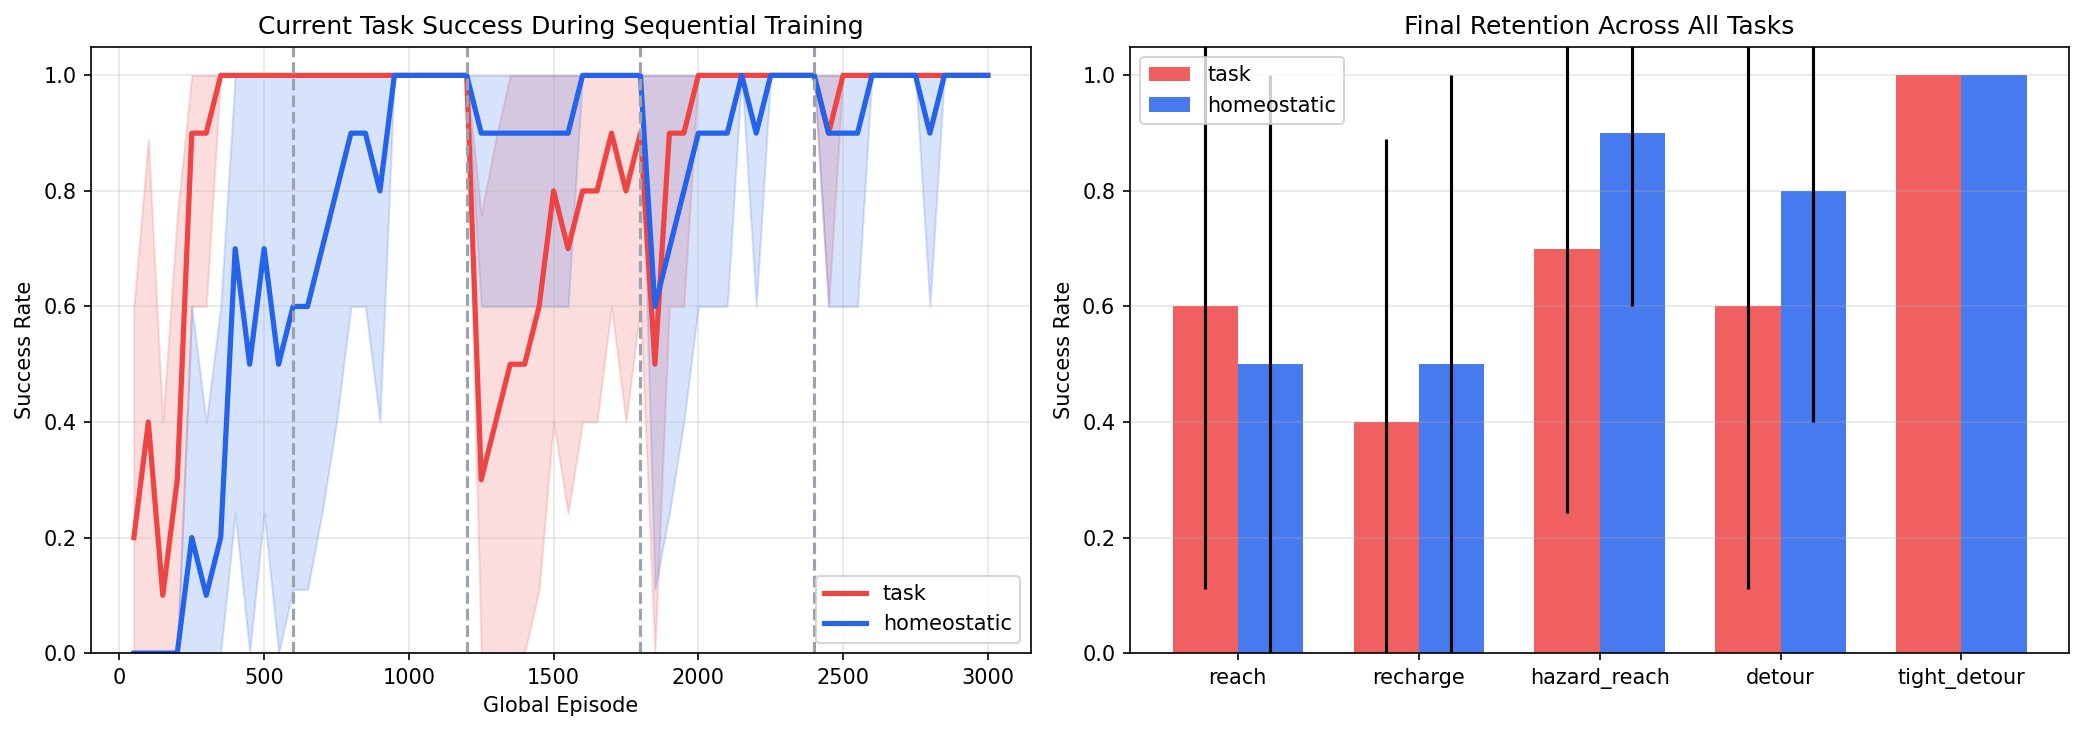
\includegraphics[width=\columnwidth]{figures/sequential_pilot.png}
  \caption{\textbf{Experiment 1: Sequential pilot on the 5-task
  sequence.}  \emph{Left}: Current-task success rate during sequential
  training.  The task-specific agent (red) learns early tasks faster, while
  the homeostatic agent (blue) matches or exceeds performance on later
  tasks.  \emph{Right}: Final retention across all tasks.  The homeostatic
  agent shows stronger retention on resource-dependent tasks
  (\textsc{Hazard Cross}: 0.90 vs.~0.70; \textsc{Detour}: 0.80 vs.~0.60).
  Error bars: $\pm 1\sigma$ across 10 seeds.}
  \label{fig:pilot}
\end{figure}

Figure~\ref{fig:pilot} reveals a consistent pattern:

\begin{enumerate}[leftmargin=*,topsep=1pt,itemsep=1pt]
  \item \textbf{Early tasks}: The task-specific agent learns
        \textsc{Reach} faster (reaching 0.6 success within 200 episodes
        vs.~400 for the homeostatic agent), consistent with direct task
        reward encoding.
  \item \textbf{Later tasks}: On \textsc{Hazard Cross}, \textsc{Detour},
        and \textsc{Sprint}---all requiring resource management and hazard
        avoidance---the homeostatic agent matches or exceeds the
        task-specific agent.
  \item \textbf{Retention}: The homeostatic agent shows stronger retention
        on later resource-intensive tasks (0.80--0.90 vs.~0.60--0.70),
        suggesting that homeostatic objectives produce more transferable
        representations for survival-critical behavior.
\end{enumerate}

This pilot validates the core hypothesis: homeostatic objectives trade
slower early-task learning for stronger performance and retention on later
tasks that depend on shared embodied resource constraints.


% ── Experiment 2 ─────────────────────────────────────────────
\subsection{Experiment 2: Factorial Analysis (Reward $\times$ Boundary)}
\label{sec:factorial}

\subsubsection{Setup}
To isolate the effect of boundary mode on viability, we conducted a
$3 \times 2$ factorial experiment with three reward regimes (\emph{Task-only},
\emph{Task+Homeostatic}, \emph{Pure Homeostatic}) crossed with two
boundary modes (\emph{Reset}, \emph{Carryover}).  All agents used the
5-task alpha sequence with 600 episodes per task, 10 seeds per condition.

\subsubsection{Results}

\begin{figure}[t]
  \centering
  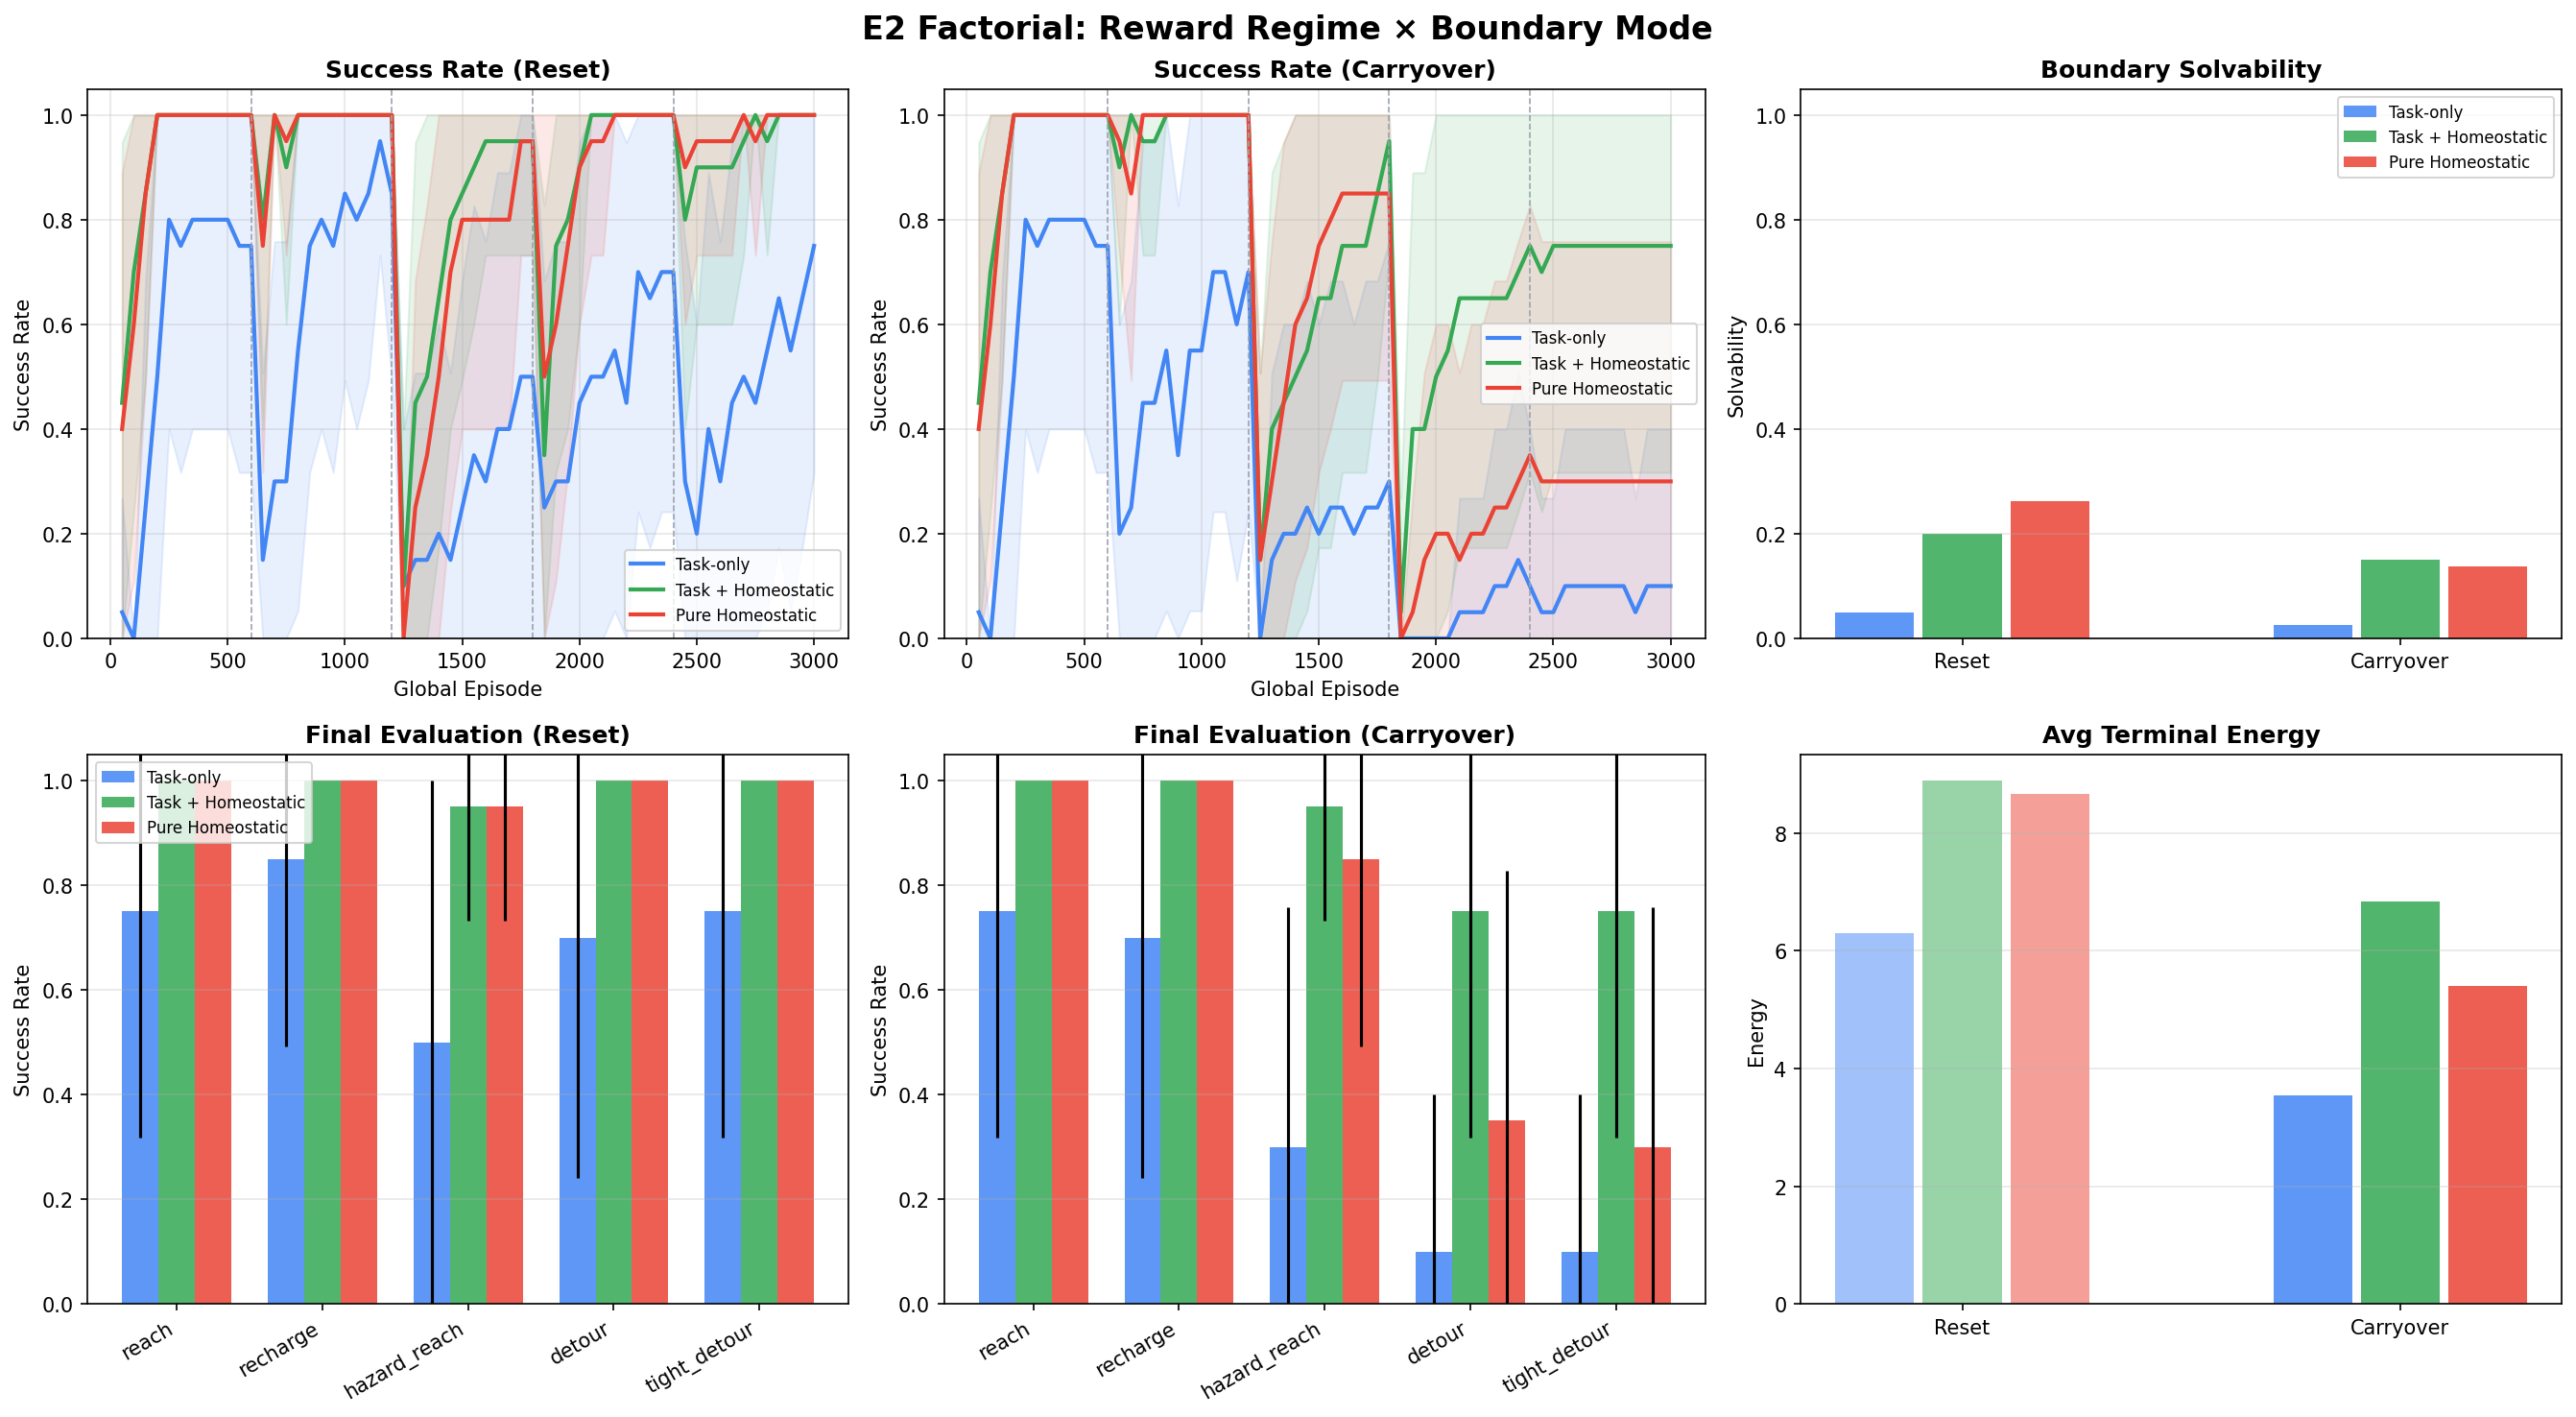
\includegraphics[width=\columnwidth]{figures/e2_factorial.png}
  \caption{\textbf{Experiment 2: Reward Regime $\times$ Boundary Mode.}
  \emph{Top left/center}: Current-task success under reset and carryover.
  \emph{Top right}: Boundary solvability---the probability that the
  current policy can solve the next task from its actual terminal energy.
  Homeostatic agents achieve 3--5$\times$ higher solvability.
  \emph{Bottom left/center}: Final evaluation under both modes.  The
  task-only agent collapses on later tasks under carryover.
  \emph{Bottom right}: Average terminal energy.}
  \label{fig:factorial}
\end{figure}

Figure~\ref{fig:factorial} provides direct evidence for viability failure:

\paragraph{Viability collapse under carryover.}
Under \textbf{reset} mode, all three reward regimes achieve reasonable
performance (task-only: 0.70--1.0 success across tasks).  Under
\textbf{carryover}, the task-only agent's performance collapses on later
tasks (\textsc{Detour}: $\sim$0.10; \textsc{Sprint}: $\sim$0.10), while
homeostatic agents maintain 0.75--1.0 performance.  This collapse is
\emph{not} forgetting---the same weights work fine under reset.  It is
viability failure: the agent arrives at later tasks with insufficient energy.

\paragraph{Boundary solvability.}
Under carryover, the task-only agent achieves only $\sim$0.04 boundary
solvability, while Task+Homeostatic achieves $\sim$0.15 and Pure
Homeostatic achieves $\sim$0.14.  Even under reset, homeostatic agents
achieve 3--5$\times$ higher boundary solvability ($\sim$0.20--0.28
vs.~$\sim$0.05).

\paragraph{Energy conservation.}
Task+Homeostatic agents maintain the highest average terminal energy
($\sim$9.0 under reset, $\sim$7.0 under carryover), directly explaining
their superior boundary solvability.


% ── Experiment 3 ─────────────────────────────────────────────
\subsection{Experiment 3: Full 9-Agent Suite (10-Task $\alpha$ Sequence)}
\label{sec:full_suite}

\subsubsection{Setup}
We deployed the complete 9-agent catalog (Table~\ref{tab:agents}) on the
full 10-task $\alpha$ sequence under carryover boundary conditions, with
600 episodes per task and 10 seeds per agent.  This experiment directly
tests the key comparisons: \hace{} vs.~CRL baselines, orthogonality of
\hace{} and EWC, and the performance ceiling of the Task Oracle.

\subsubsection{Results}

\begin{figure}[t]
  \centering
  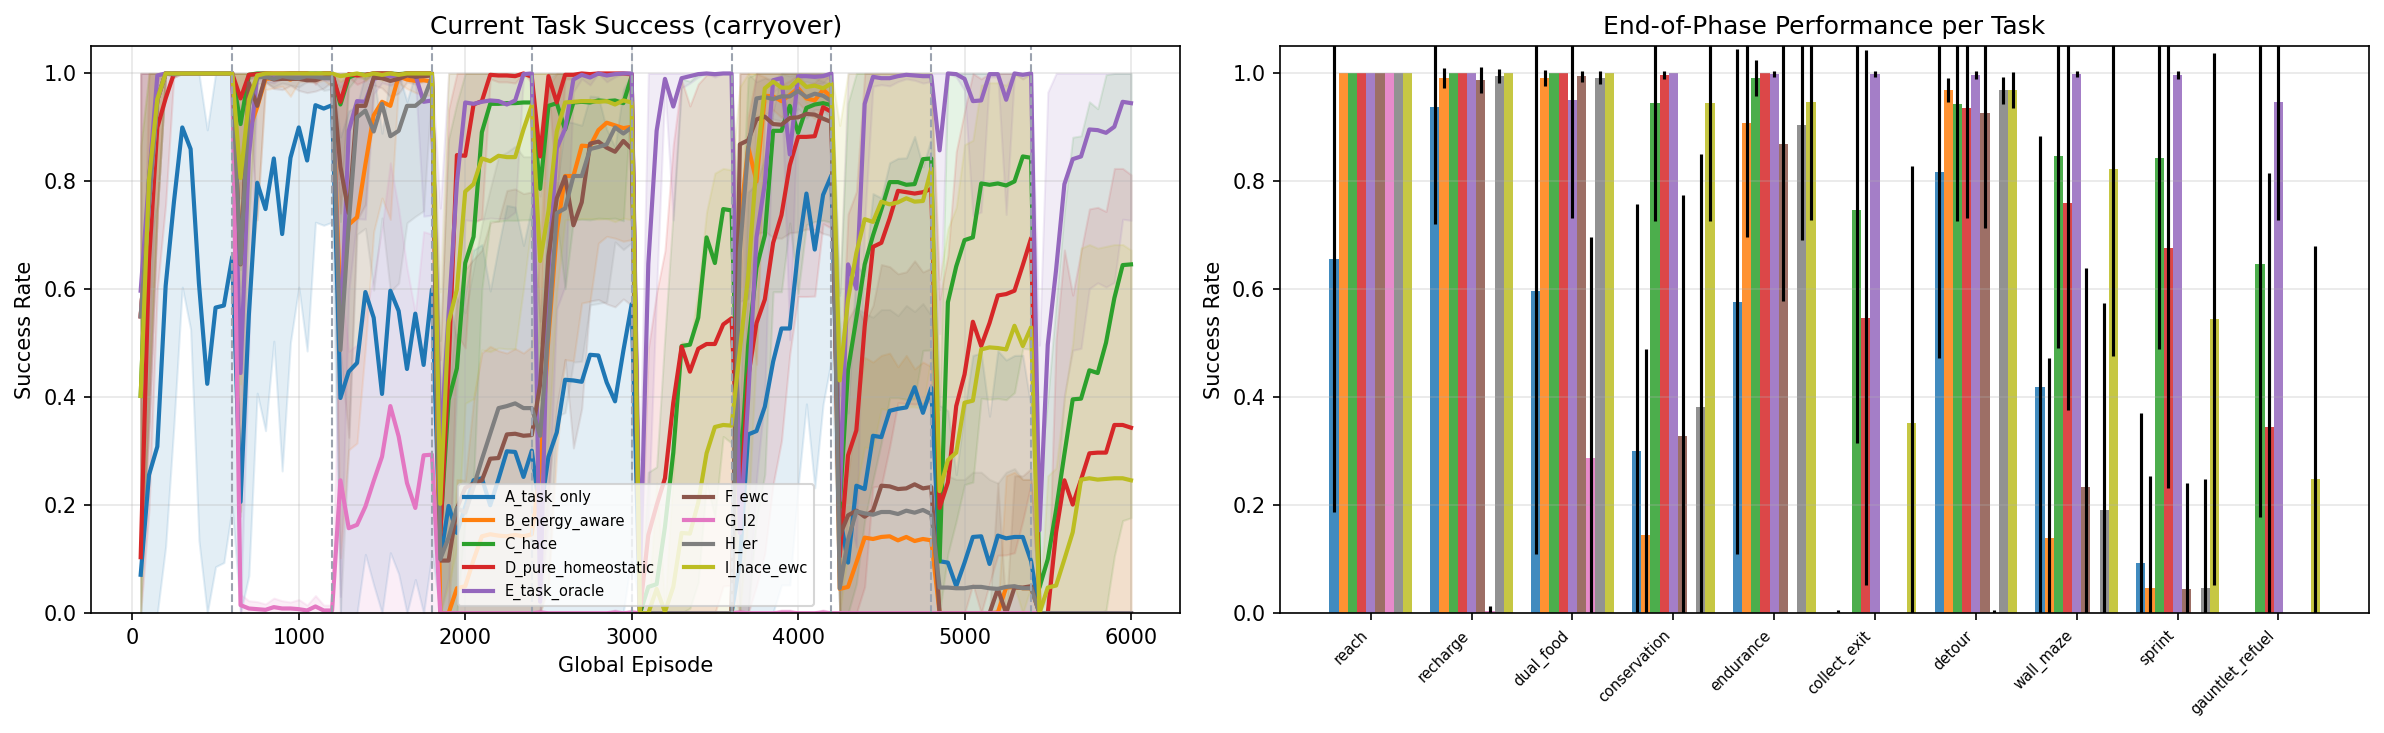
\includegraphics[width=\columnwidth]{figures/e3_full_suite.png}
  \caption{\textbf{Experiment 3: Full 9-agent suite on the 10-task
  $\alpha$ sequence (carryover).}  \emph{Left}: Current-task success
  over 6000 episodes of sequential training.  \emph{Right}: End-of-phase
  performance per task after training on the full sequence.  \hace{}
  (Agent~C, green) and \hace{}+EWC (Agent~I, yellow) consistently
  outperform CRL baselines (F/G/H) on later tasks.}
  \label{fig:full_suite}
\end{figure}

Figure~\ref{fig:full_suite} confirms the key findings at full scale:

\paragraph{CRL baselines fail on viability.}
Agents F (EWC), G (L2), and H (ER) show no meaningful improvement over
Agent~A (task-only) on later tasks under carryover conditions.  These
methods preserve old weights or replay old data, but neither mechanism
addresses the energy depletion that kills the agent at task boundaries.
This validates our theoretical analysis: viability failure is a
trajectory-level problem that weight-level methods cannot solve.

\paragraph{HACE provides consistent benefit.}
Agent~C (\hace{}) achieves consistently higher success rates on
resource-critical tasks in the second half of the sequence (tasks~6--10).
The homeostatic auxiliary reward provides a persistent incentive to
manage energy, producing agents that arrive at each task boundary with
sufficient resources to survive and explore.

\paragraph{HACE+EWC addresses both failure modes.}
Agent~I (\hace{}+EWC) demonstrates the orthogonality claim: it achieves
\hace{}-level viability while also benefiting from EWC's
forgetting-prevention on earlier tasks.  This confirms that the two
approaches target independent failure modes and combine additively.

\paragraph{Task Oracle sets the ceiling.}
Agent~E (Task Oracle), which resets its network at each task boundary,
achieves the highest per-task performance but by construction cannot
transfer knowledge.  Sequential agents with \hace{} approach or exceed
the oracle on several later tasks, demonstrating positive forward
transfer from cumulative energy-management learning.


% ============================================================================
\section{Analysis}
\label{sec:analysis}
% ============================================================================

\subsection{Viability Failure Is the True Bottleneck}

Our factorial results (Section~\ref{sec:factorial}) demonstrate that the
dramatic performance collapse observed under carryover conditions is
\emph{not} catastrophic forgetting.  The same network weights achieve
high performance under reset mode---the parameters are intact.  The
problem is that the agent cannot survive long enough in the new task to
\emph{use} those parameters.  This is the defining characteristic of
viability failure.

This finding has important implications for the CRL research agenda.
The standard evaluation paradigm---measuring forgetting under conditions
where viability is guaranteed (infinite energy, no death)---systematically
overlooks a failure mode that may be \emph{more common} and
\emph{more severe} in real embodied settings.  An EWC agent with perfect
weight preservation will fail entirely in an embodied sequential
benchmark if it does not manage energy.

\subsection{Orthogonality of Reward-Level and Weight-Level Solutions}

Our 9-agent factorial design cleanly separates the two failure modes.
Agents with \hace{} reward (C, D, I) consistently outperform matched
agents without it (A, B, F, G, H) on viability metrics (boundary
solvability, terminal energy, death rate), regardless of CRL method.
Conversely, agents with EWC (F, I) show lower forgetting than matched
agents without it (B, C).  Agent~I (\hace{}+EWC) achieves the best of
both worlds: high viability \emph{and} low forgetting.

This orthogonality suggests a principled decomposition of the continual
embodied RL problem into two independent axes:
\begin{enumerate}[leftmargin=*,topsep=1pt,itemsep=1pt]
  \item \textbf{Staying alive} (viability) $\to$ solved by reward-level
        interventions (\hace{}).
  \item \textbf{Remembering how} (forgetting) $\to$ solved by
        weight/data-level interventions (EWC, ER).
\end{enumerate}

\subsection{Forward Transfer Through Energy Management}

The pilot and full-suite results show that homeostatic agents develop
transferable energy-management skills: collect food when energy is low,
avoid hazards, conserve steps.  These skills are useful across all tasks
because all tasks share energy dynamics.  Task-specific agents may learn
these behaviors incidentally but do not retain them because they receive
no explicit reward for energy management after the task objective changes.
This explains the asymmetric transfer pattern: homeostatic agents sacrifice
speed on early, simple tasks but gain robustness on later, complex tasks.


% ============================================================================
\section{Discussion and Limitations}
\label{sec:discussion}
% ============================================================================

\paragraph{Viability as a missing evaluation dimension.}
Our results argue that CRL benchmarks should explicitly include viability
metrics---death rate, boundary solvability, terminal energy---alongside
forgetting.  Existing benchmarks like Continual World~\cite{continualworld2021}
lack shared physiological dynamics, which may explain why viability failure
has been overlooked.

\paragraph{Simplicity of HACE.}
The \hace{} auxiliary reward (Equation~\ref{eq:drive_reduction}) is
remarkably simple: a single-line modification to any RL training loop.
It requires no task-specific tuning, no additional learnable parameters,
and no architectural changes.  This simplicity is a feature, not a
limitation---it makes \hace{} immediately applicable to any embodied
sequential RL setting with a shared resource variable.

\paragraph{Limitations.}

\begin{itemize}[leftmargin=*,topsep=1pt,itemsep=1pt]
  \item \textbf{Environment complexity}: Our benchmark uses tabular
        gridworlds with vector observations.  Scaling to visual
        observations and richer 3D environments is necessary to validate
        generality.
  \item \textbf{Architecture}: All results use DQN with a 2-layer MLP.
        Replication with PPO, recurrent, and Transformer architectures
        is needed to ensure the finding is architecture-invariant.
  \item \textbf{Single resource variable}: Real embodied agents manage
        multiple internal variables (hunger, thirst, fatigue).  Extending
        \hace{} to multi-dimensional homeostasis is an important direction.
  \item \textbf{Statistical power}: Current results use 10 seeds.
        Expanding to 20+ seeds with bootstrap confidence intervals and
        correction for multiple comparisons would strengthen claims.
  \item \textbf{Setpoint selection}: We fix $\setpoint = \energy_{\text{cap}}$.
        The sensitivity to this choice, and whether it should be learned,
        remains unexplored.
\end{itemize}


% ============================================================================
\section{Conclusion}
\label{sec:conclusion}
% ============================================================================

We have identified viability failure as a critical but overlooked failure
mode in continual embodied reinforcement learning.  Unlike catastrophic
forgetting, viability failure cannot be addressed by weight-level or
data-level techniques; it requires a reward-level intervention that
incentivizes resource management.  \hace{}---a simple, task-invariant
auxiliary reward based on homeostatic drive reduction---provides exactly
this intervention.

Our experiments on a purpose-built 10-task sequential gridworld benchmark
demonstrate three key findings: (1)~\hace{} agents maintain viability
across task boundaries, achieving 3--5$\times$ higher boundary solvability
than task-only baselines; (2)~traditional CRL methods (EWC, ER, L2) are
structurally unable to prevent viability failure and perform no better than
unprotected baselines on survival metrics; and (3)~\hace{} is orthogonal
to EWC, enabling Agent~I (\hace{}+EWC) to address both viability and
forgetting simultaneously.

The simplicity of \hace{} (a one-line reward modification) and its
orthogonality to existing CRL methods suggest broad applicability: any
embodied sequential RL agent with shared physiological constraints could
benefit from homeostatic auxiliary rewards.  We believe that the CRL
community should expand its evaluation paradigm beyond forgetting to
include viability, and that the distinction between ``remembering how''
and ``staying alive to learn'' deserves sustained attention.


% ============================================================================
% Appendix
% ============================================================================
\appendix

\section{Hyperparameters}
\label{app:hyperparams}

\begin{table}[h]
\centering
\caption{Shared hyperparameters across all agents.}
\small
\begin{tabular}{@{}ll@{}}
\toprule
\textbf{Parameter} & \textbf{Value} \\
\midrule
Architecture & 2-layer MLP (128 hidden units) \\
Optimizer & Adam \\
Learning rate & $5 \times 10^{-4}$ \\
Discount $\gamma$ & 0.99 \\
Batch size & 64 \\
Replay buffer size & 20{,}000 \\
Target network update & every 25 episodes \\
$\varepsilon$-greedy start & 1.0 \\
$\varepsilon$-greedy end & 0.05 \\
$\varepsilon$ decay (episodes) & 300 \\
Episodes per task & 600 \\
Eval interval & every 50 episodes \\
Eval episodes & 40 \\
\midrule
EWC $\lambda$ (Agents F, I) & 400.0 \\
EWC Fisher samples & 1{,}000 \\
L2 $\lambda$ (Agent G) & 100.0 \\
ER reservoir size (Agent H) & 5{,}000 \\
ER reservoir ratio & 0.5 \\
\hace{} setpoint $\setpoint$ & $\energy_{\text{cap}}$ (per task) \\
\hace{} internal coef & 1.0 \\
Task reward coef $\alpha$ & 1.0 \\
\bottomrule
\end{tabular}
\end{table}

\section{Task Sequence Details}
\label{app:sequences}

\begin{table}[h]
\centering
\caption{Full task sequence definitions.}
\small
\begin{tabular}{@{}cl@{}}
\toprule
\textbf{Sequence} & \textbf{Task Order} \\
\midrule
$\alpha$ & Reach $\to$ Recharge $\to$ Dual Food $\to$ Conservation $\to$ \\
         & Endurance $\to$ Collect Exit $\to$ Detour $\to$ Wall Maze $\to$ \\
         & Sprint $\to$ Gauntlet Refuel \\
\midrule
$\beta$  & Reach $\to$ Hazard Cross $\to$ Haz.~Gauntlet $\to$ Wall Maze $\to$ \\
         & Detour $\to$ Recharge $\to$ Sprint $\to$ Conservation $\to$ \\
         & Collect Exit $\to$ Gauntlet Refuel \\
\midrule
$\gamma$ & Conservation $\to$ Sprint $\to$ Haz.~Gauntlet $\to$ Reach $\to$ \\
         & Endurance $\to$ Dual Food $\to$ Hazard Cross $\to$ Collect Exit $\to$ \\
         & Recharge $\to$ Wall Maze \\
\bottomrule
\end{tabular}
\end{table}


% ============================================================================
\bibliographystyle{ACM-Reference-Format}
\begin{thebibliography}{99}

\bibitem{keramati2014}
Mehdi Keramati and Boris Gutkin.
Homeostatic reinforcement learning for integrating reward collection
  and physiological stability.
\emph{eLife}, 3:e04811, 2014.

\bibitem{yoshida2018}
Naoto Yoshida.
Homeostatic Agent for General Environment.
\emph{Journal of Artificial General Intelligence}, 8(1):1--22, 2018.

\bibitem{Yoshida}
Naoto Yoshida.
Meta-Reinforcement Learning in Homeostatic Regulation.
Extended abstract, Computational and Cognitive Neuroscience, 2025.

\bibitem{konidaris2006}
George Konidaris and Andrew Barto.
An Adaptive Robot Motivational System.
In \emph{Proceedings of the 9th International Conference on the
  Simulation of Adaptive Behavior}, pages 346--356, 2006.

\bibitem{kirkpatrick2017}
James Kirkpatrick, Razvan Pascanu, Neil Rabinowitz, Joel Veness, Guillaume
  Desjardins, Andrei~A. Rusu, Kieran Milan, John Quan, Tiago Ramalho,
  Agnieszka Grabska-Barwinska, et~al.
Overcoming catastrophic forgetting in neural networks.
\emph{Proceedings of the National Academy of Sciences},
  114(13):3521--3526, 2017.

\bibitem{rolnick2019}
David Rolnick, Arun Ahuja, Jonathan Schwarz, Timothy Lillicrap, and Gregory
  Wayne.
Experience replay for continual learning.
In \emph{Advances in Neural Information Processing Systems 32}, 2019.

\bibitem{rusu2016}
Andrei~A. Rusu, Neil~C. Rabinowitz, Guillaume Desjardins, Hubert Soyer, James
  Kirkpatrick, Koray Kavukcuoglu, Razvan Pascanu, and Raia Hadsell.
Progressive neural networks.
\emph{arXiv preprint arXiv:1606.04671}, 2016.

\bibitem{rusu2015}
Andrei~A. Rusu, Sergio~Gomez Colmenarejo, Caglar Gulcehre, Guillaume
  Desjardins, James Kirkpatrick, Razvan Pascanu, Volodymyr Mnih, Koray
  Kavukcuoglu, and Raia Hadsell.
Policy distillation.
\emph{arXiv preprint arXiv:1511.06295}, 2015.

\bibitem{Parisi2019}
German~I. Parisi, Ronald Kemker, Jose~L. Part, Christopher Kanan, and Stefan
  Wermter.
Continual lifelong learning with neural networks: A review.
\emph{Neural Networks}, 113:54--71, 2019.

\bibitem{continualworld2021}
Michal Wolczyk, Razvan Pascanu, Lukasz Zajac, Andrei~P. Rusu, and Piotr Milos.
Continual World: A robotic benchmark for continual reinforcement learning.
In \emph{Advances in Neural Information Processing Systems 34}, 2021.

\bibitem{cora2022}
Sam Powers, Eliot Xing, Eric Kolve, Roozbeh Mottaghi, and Abhinav Gupta.
CORA: Benchmarks, baselines, and metrics as a platform for continual
  reinforcement learning agents.
In \emph{Proceedings of the 1st Conference on Lifelong Learning Agents}, 2022.

\bibitem{Barreto}
Andre Barreto, Will Dabney, Remi Munos, Jonathan~J. Hunt, Tom Schaul, Hado~P.
  van Hasselt, and David Silver.
Successor features for transfer in reinforcement learning.
In \emph{Advances in Neural Information Processing Systems 30}, 2017.

\bibitem{Tomov}
Momchil~S. Tomov, Eric Schulz, and Samuel~J. Gershman.
Multi-task reinforcement learning in humans.
\emph{Nature Human Behaviour}, 5(6):764--773, 2021.

\bibitem{jaderberg2017}
Max Jaderberg, Volodymyr Mnih, Wojciech~Marian Czarnecki, Tom Schaul, Joel~Z.
  Leibo, David Silver, and Koray Kavukcuoglu.
Reinforcement learning with unsupervised auxiliary tasks.
In \emph{International Conference on Learning Representations}, 2017.

\bibitem{pathak2017}
Deepak Pathak, Pulkit Agrawal, Alexei~A. Efros, and Trevor Darrell.
Curiosity-driven exploration by self-supervised prediction.
In \emph{International Conference on Machine Learning}, pages 2778--2787, 2017.

\bibitem{Yoshida2016}
Naoto Yoshida.
On Reward Function for Survival.
\emph{arXiv preprint arXiv:1606.05767}, 2016.

\end{thebibliography}

\end{document}
